%\documentclass[english,twoside]{article}
\documentclass[english,twoside]{labmanual} 
%labmanual.cls is a modified version of article.cls, tweaked to handle \part{} differently

%% LyX 1.1 created some parts of this file.  For more info, see http://www.lyx.org/.
%% Do not edit unless you really know what you are doing.

\usepackage[T1]{fontenc}
\usepackage[nomarginpar]{geometry}
\usepackage{tocloft} %Allow us to leave page numbers for Parts out of table of contents
\cftpagenumbersoff{part} %No page numbers for Parts out of table of contents
\renewcommand{\cftsecdotsep}{\cftsubsecdotsep}
%\usepackage{newclude} %Allows use of /include*{}
%DANGER DANGER: newclude is NOT compatible with package xr, used for external references.
\geometry{verbose,letterpaper}
\usepackage{fancyhdr}
\usepackage{babel}
\setlength\parskip{\medskipamount}
\setlength\parindent{0pt}
\usepackage{graphicx}
\usepackage{wrapfig}
%\usepackage{epstopdf} %this package apparently allows pdflatex to work on this document, since all we use are eps figures.
\usepackage{comment}
\usepackage{esvect}
\usepackage{amsmath} %uncommented by MT 5/2015, used in "E near charged rod"
\usepackage{mathtools} %added by MT 6/2015, for access to dcases environment in finding_v_from_e
\usepackage{tabularx} %added by MT 6/2015, for fixed width columns, used in rc_circuits
\usepackage{microtype}
\usepackage{titlesec}
\usepackage{xr}

%For fixed width columns:
\newcolumntype{L}[1]{>{\raggedright\arraybackslash}p{#1}}
\newcolumntype{C}[1]{>{\centering\arraybackslash}p{#1}}
\newcolumntype{R}[1]{>{\raggedleft\arraybackslash}p{#1}}


\addtolength{\oddsidemargin}{1.3cm} %without these two lines, larger margin is on the OUTSIDE.  We want the larger edge on the INSIDE, to allow room for the three hole punches
\addtolength{\evensidemargin}{-1.3cm}

\setlength\topmargin{0.2in}
\addtolength{\hoffset}{-1.0cm}
\addtolength{\textwidth}{2.0cm}
\addtolength{\voffset}{-1.5cm} %This line is apparently needed on some versions of MikTex XeLatex.  Comment out if your pages appear shifted too high.
\addtolength{\textheight}{3.5cm}
% define a strut for extra vertical space in tables.
\newcommand{\hi}{\rule[-2mm]{0mm}{6mm}}

\pagestyle{fancy}
%\fancyhead[LE,RO]{\slshape \rightmark} %This is the default for fancy page style
%\fancyhead[LO,RE]{\slshape \leftmark}
\fancyhead[LO,RE]{\slshape \rightmark} 
\fancyhead[LE,RO]{\slshape \leftmark} % Reversed LE, RO to  LO,RE to make headers come out correctly on even/odd pages



%%%%%%%%%%%%%%%%%%%%%%%%%%%%%% LyX specific LaTeX commands.
\providecommand{\LyX}{L\kern-.1667em\lower.25em\hbox{Y}\kern-.125emX\@}
\newenvironment{LyXParagraphIndent}[1]%
{
  \begin{list}{}{%
    \setlength\topsep{0pt}%
    \addtolength{\leftmargin}{#1}
    \setlength\parsep{0pt plus 1pt}%
  }
  \item[]
}
{\end{list}}
%% Special footnote code from the package 'stblftnt.sty'
%% Author: Robin Fairbairns -- Last revised Dec 13 1996
\makeatletter
\let\SF@@footnote\footnote
\def\footnote{\ifx\protect\@typeset@protect
    \expandafter\SF@@footnote
  \else
    \expandafter\SF@gobble@opt
  \fi
}
\expandafter\def\csname SF@gobble@opt \endcsname{\@ifnextchar[%]
  \SF@gobble@twobracket
  \@gobble
}
\edef\SF@gobble@opt{\noexpand\protect
  \expandafter\noexpand\csname SF@gobble@opt \endcsname}
\def\SF@gobble@twobracket[#1]#2{}
\makeatother


%I make use of some latex features to manage the section numbers. To use those you have to insert the following lines into the latex preamble (before the %"\begin{document}" command).

% two new commands to do labelling. - gpg 12/4/13
\newcommand{\customlabel}[2]{%
\protected@write \@auxout {}{\string \newlabel {#1}{{#2}{}}}}

\newcommand{\actlabel}[1]{%
\protected@write \@auxout {}{\string \newlabel {#1}{{\arabic{activity}}{}}}}

\newcommand{\makelabheader}
%{Name: \rule{2.0in}{0.1pt}\hfill{}Section: \rule{1.0in}{0.1pt}\hfill{}Date: \rule{1.0in}{0.1pt}}
{Name: \rule{2.0in}{0.1pt}\hfill{}Lab Partner(s): \rule{3.0in}{0.1pt}}

%\newcommand{\dir131}{../../131/StudentGuideModule1} %This does not work, because commands can only be made of numeric characters, not numbers.

%A new command for putting a box around a paragraph:
\newenvironment{newboxed} %maybe there's a better way to do this.  I just cribbed from the web. --MT
    {\begin{center}
    \begin{tabular}{|p{0.9\textwidth}|}
    \hline\\
    }
    { 
    \\\\\hline
    \end{tabular} 
    \end{center}
    }

\newcounter{activity}

\newcommand{\answerspace}[1]{\vspace*{#1 plus #1}}

\newif\ifincludealllabs
\newcommand{\includelab}[2]{
	\ifnum#1=1
		\include{#2}
	\else {
		\ifincludealllabs
		 	\include{#2}
		\fi}
	\fi
}
 %all general latex packages, commands, and definitions now here.
\externaldocument{master}

%syntax: \includeonly{lab1,lab2,lab3} with no spaces after the commas.
%\includeonly{biot_savart_law/biot_savart_law, charge_density/charge_density,eoverm/eoverm }
%DANGER: The includeonly statement will make a document that does NOT have sequential page numbers.

\newcommand{\supplementmark}{MT}

\titleformat{\section}{\normalfont\Large\bfseries}{\supplementmark \thesection}{1em}{}
\fancyhead[LO,RE]{\slshape \rightmark} 
\fancyhead[LE,RO]{\slshape \supplementmark \leftmark} % Reversed LE, RO to  LO,RE to make headers come out correctly on even/odd 

\begin{document}

\setcounter{page}{165}  %Set this to desired first page
\setcounter{section}{38} %set this to desired first section number MINUS ONE

%--------------------------------------------
%Put include statements for labs below here.
\section{How to Tune a Piano}

\instructornote{%
By Matt, added to manual Spring 2017.  Time: $\sim$20 minutes

This lab is definitely off the beaten path, but some students think it's fun, and it's short.

The Wikipedia page for ``musical tuning'' includes some examples of a Bach prelude played in different tunings (``just intonation'' and ``even temperament'') and I always play those to the class.  It's really obvious how ``just temperament'' leads to a few chords that sound really badly out of tune!
}

\makelabheader %(Space for student name, etc., defined in master.tex)

\bigskip
\textbf{Apparatus}
%\vspace{-\parskip}
\begin{itemize}[nosep]
\item piano\_tuning.xlsx spreadsheet file
\end{itemize}

\medskip
\textbf{Introduction}

Tuning musical instruments is probably not something you think about every day.  But it turns out that what counts as ``in tune'' for a piano is not as straightforward as it seems.  There are lots of possible ways to tune the notes on a piano, all of which sound subtly different.

\medskip
\textbf{A C major chord}

(a) Open the spreadsheet piano\_tuning.xlsx in Excel.  Your first job is to calculate in column F the exact frequencies for the notes in a C major chord: C, E, G, and another high C. 

\vspace{-0.25in}

%\medskip
\hspace{1.10in}\raisebox{-0.25in}{130.8~Hz}

\vspace{-0.15in}
\hfill{}
Low C ($f_0$): \rule{.7in}{0.1pt}\hfill{}
E ($\frac{5}{4}f_0$): \rule{.7in}{0.1pt}\hfill{}
G ($\frac{3}{2}f_0$): \rule{.7in}{0.1pt}\hfill{}
high C ($2f_0$): \rule{.7in}{0.1pt}\hfill{}

The values you have just calculated probably sound the most ``in tune'' to your ears.

\medskip
\textbf{Just Intonation}

(b) Now you will fill in column G in the spreadsheet using a scheme of simple whole number ratios called ``just intonation.'' In this scheme, 
\begin{itemize}[nosep]
\item Each pair of notes that are seven notes away from each other on the keyboard (a ``perfect fifth'', like from C to G) has a frequency ratio of 3:2.
\item Each pair of notes that are twelve notes away from each other (an ``octave'', like from a low C to a higher C) has a frequency ratio of 2:1.  
\end{itemize}
Fill in the frequencies of column G, starting with the low C and alternating between going seven notes up and five notes down.  (For five notes down, the frequency ratio is 3:4, the same as going up by seven notes twice, then down by an octave.) For convenience, the order to calculate the frequencies is given in column H.)

(c) What is the frequency of the high C? Is it exactly twice the frequency of the low C, 130.8~Hz?
\answerspace{0.3in}

(d) Are the frequencies for the C major chord (C, E, G) exactly the same as you calculated in part (a)?
\answerspace{0.3in}

\textbf{Even Temperament}

Using the ``just intonation'' scheme you just calculated, the high C would be moved back to 261.6 Hz, which would preserve the 2:1 frequency ratio between the two C's, but would make some other pairs of notes sound \textit{awful} to our ears!  A clever alternative tuning that avoids this, called ``even temperament,'' was invented around the time of Johann Sebastian Bach.  The rule is simple:
\begin{itemize}[nosep]
\item Each pair of adjacent notes (like C to C\#) has a frequency ratio of $\sqrt[12]{2}:1$.
\end{itemize}

(e) Fill in the frequencies of column I, starting with the low C.  (The value of $\sqrt[12]{2}$ is given in cell A1.)

(f) Does the last C come out to exactly 261.6 Hz?
\answerspace{0.3in}

(g) Do the frequencies for the C major chord exactly match part (a)?  Are they at least closer than with ``just intonation?''
\answerspace{0.3in}

\section{Introduction to Electric Potential}
\label{potential_intro}

\instructornote{%
By Matt, Spring 2017.  Time: 80 minutes in class, even with Activity 0 done previously as homework.

Matt sez: I recommend assigning some ``review homework'' on the relationship between $F$ and $U$ from previous chapters before doing this lab.  I also assign Activity 0 as homework, asking students to start the lab by checking their answers for Activity 0 with their lab partners.  Even so, students struggle mightily with signs in Activity 1.
}

\makelabheader %(Space for student name, etc., defined in master.tex)

\bigskip

\textbf{Introduction} 

In this lab, we'll start by reviewing the ideas of force, work, and potential energy from physics 131.  Then we'll define a new, handy quantity called the ``electric potential'' that's one of the key ideas in physics 132.

\bigskip

\textbf{Activity 0: Review of Force and Potential Energy from Physics 131}\footnote{This activity could be done as homework before the rest of the lab.}

In your previous physics class, you learned that the work $W$ done on an object by a uniform force $F$ is given by $W=\vv{F} \cdot \vv{{\scriptstyle \Delta} s}$, where $\vv{{\scriptstyle \Delta} s}$ is the displacement of the object.

\begin{enumerate}[labparts]

\item Suppose that a ball moves along each of the four numbered paths shown below.  For each one, is the work done by the force of gravity \textit{positive}, \textit{negative}, or \textit{zero}? \label{part_potential_intro_grav_work} 
\begin{center}
\vspace{0.1in}
\includegraphics{potential_intro/activity_1_figs/gravity_paths.eps}
\vspace{0.1in}
\end{center}

For forces like gravity that only depend on the position of the object, you learned that instead of treating the force as  ``external'' (from outside the system) it's sometimes handy to include the source of the force (the Earth, in this case) as a part of the system, defining a potential energy $U$ so that
$$\Delta U \equiv -W.$$

\item For each of the four paths in the figure in part \ref{part_potential_intro_grav_work}, state whether the change in gravitational potential energy $\Delta U$ of the system is \textit{positive}, \textit{negative}, or \textit{zero}.
\begin{center}
\vspace{0.05in}
\includegraphics{potential_intro/activity_1_figs/gravity_potentials.eps}
\vspace{0.05in}
\end{center}

\textit{Helpful hint: It's easy to make a careless algebraic mistake with a sign, so always check yourself by telling yourself a little story like this: if you were to reach into the system with your hand and lift a ball along path 2, the external force of your hand would be doing \textit{positive} work on the system---that's why you get tired.  The calories you burned went someplace, and they went to \textit{increasing} the gravitational potential energy of the system. }

\pagebreak[3]

\item For non-uniform forces (that is, forces that change with position), the work done by a force is given by 
$$W=\int{\vv{F} \cdot \vv{ds}}$$
which reduces to just $W=\int{F ds}$ in one dimension.  The diagram below shows the resulting general relationship between force $\vv{F}$ and potential energy $U$.  Complete the equation on the right showing how to find the force if you know the potential energy $U$.  (Yep, it'll be the opposite of an integral.)
\begin{center}
\vspace{-0.1in}
\includegraphics{potential_intro/concept_map_figs/concept_map_F_and_U_blank_squish.eps}
\end{center}

%\end{enumerate}

%\begin{minipage}{0.64\textwidth}
%\begin{enumerate}[resume,wide, label=(\emph{\alph*})]
\item As an example, consider a mass $m$ on a spring with a spring constant $k$ in the figure to the right.  For simplicity, we'll assume the surface is frictionless, and that the equilibrium position of the mass is at $x=0$.  
Draw a graph of the force $F$ of the spring on the mass, as a function of its position $x$.  
(Hints: this is your old friend, Hooke's law.  Also, think about the signs: if the mass is at a positive $x$, is the force of the spring pushing it in the positive direction or the negative direction?)
%\end{enumerate}
%\end{minipage}
%\begin{minipage}{0.34\textwidth}
%\includegraphics[width=1.0\textwidth]{potential_intro/activity_1_figs/mass_on_spring.eps}
%\end{minipage}

\begin{center}
%\vspace{-0.1in}
%\includegraphics{potential_intro/activity_1_figs/F_axes.eps}
\begin{lab_axis}[lab_noticks_4quads,
	width={3.0in}, height={1.7in},
	xlabel={$x$},
	ylabel={$F$},
	]
\end{lab_axis}
\hspace{0.5in}
\raisebox{0.3in}{\includegraphics[scale=0.8]{potential_intro/activity_1_figs/mass_on_spring.eps}}
\end{center}

%\begin{enumerate}[resume*,start=5] %this hard-codes the start at letter e.  Somehow it always restarted at d before.

%\newpage

\item From the force law $F(x)$ you just graphed, write an expression $U(x)$ for the potential energy of the system as a function of the position of the mass.  Sketch a graph of $U(x)$ on the axes below.
\begin{center}
%\vspace{-0.1in}
%\includegraphics{potential_intro/activity_1_figs/U_axes.eps}
\begin{lab_axis}[lab_noticks_4quads,
	width={3.0in}, height={1.5in},
	xlabel={$x$},
	ylabel={$U$},
	ymin=-0.3,
	]
\end{lab_axis}
\hspace{1.05in}
\raisebox{0.3in}{$U(x)=$}
\hspace*{1.0in}
\end{center}

Note that when you integrate $F(x)$, you should include an integration constant $+C$.  It doesn't matter what you pick for $C$; you can add any constant you want to $U(x)$, because we only ever care about \textit{differences} $\Delta U$ anyway.  (It's the same as how you can define gravitational potential energy so that $U_{\rm grav}=0$ is at sea level or the top of your lab table.)  The easiest choice here is probably $C=0$.
\end{enumerate}

\pagebreak[2]
\textbf{Activity 1: Electric Potential Energy}

Now that we've reviewed gravitational potential energy $U_{\rm grav}$ and the potential energy of a spring $U_{\rm spring}$, let's take a look at an example of electric potential energy.  

\begin{enumerate}[labparts]

\item The figure below shows a region of uniform electric field $E_0$.  If a \textit{positively} charged particle $+q$ moves along the path shown with the dashed line, is the change in potential energy of the system \textit{positive}, \textit{negative}, or \textit{zero?}  Compare with the gravitational example on page \pageref{part_potential_intro_grav_work}.
\begin{center}
%\vspace{0.1in}
\includegraphics{potential_intro/activity_2_figs/uniform_E_field.eps}
%\vspace{0.1in}
\end{center}


\item What is the magnitude of the electric force $\vv{F}$ on the charged particle?
\answerspace{0.3in}

\item By integrating the force above, write a function for the potential energy $U(x)$ for the particle in the field.  Be sure to include an integration constant, $+C$.
\answerspace{0.3in}

\item Suppose that the particle's initial position is at $x=0$, and we want to define the potential energy $U(x)$ so that $U=0$ at $x=0$.  What value should you choose for the integration constant $C$?
\answerspace{0.3in}

\item Sketch a qualitative graph of the potential energy function $U(x)$ you just found.
%\begin{center}
%\vspace{-0.1in}
%\includegraphics{potential_intro/activity_2_figs/U_axes_2.eps}
%\vspace{-0.1in}
%\end{center}
\begin{lab_axis}*[lab_noticks_4quads,
	width={3.0in}, height={1.7in},
	xlabel={$x$},
	ylabel={$U$},
	]
\end{lab_axis}

\item Sketch a qualitative graph of what the potential energy function $U(x)$ would look like if the particle were \textit{negatively} charged.

%\begin{center}
%\vspace{-0.1in}
%\includegraphics{potential_intro/activity_2_figs/U_axes_2.eps}
%\vspace{-0.1in}
%\end{center}
\begin{lab_axis}*[lab_noticks_4quads,
	width={3.0in}, height={1.7in},
	xlabel={$x$},
	ylabel={$U$},
	]
\end{lab_axis}

\end{enumerate}

\pagebreak[3]
\textbf{Activity 2: A First Look at Electric Potential \textit{V}}

\textbf{Why Electric Field Is Useful...}


Suppose a bunch of electric charges ($Q_1$, $Q_2$, etc.) are nailed down so they don't move.  If you take an additional charge $q$ out of your pocket and place it in a specific location, there will be an electric force on it from the nailed down charges.  You could calculate the force directly, using Coulomb's law, for instance.  
\begin{wrapfigure}[8]{r}{0.27\textwidth}
\begin{center}
\vspace{-0.3 in}
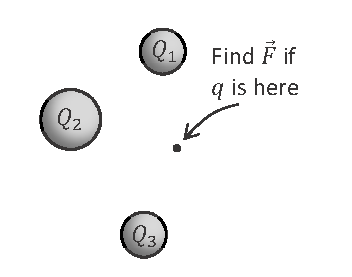
\includegraphics[scale=0.8]{potential_intro/activity_3_figs/charge_from_pocket.eps}
\end{center}
\end{wrapfigure}


But the size of the force depends on what charge $q$ you pull from your pocket, and you might not want to recalculate the force from scratch for every possible charge you could pull out.  Instead, you can calculate the electric field $\vv{E}$ due to the fixed charges, and then find the force on any charge $q$ using $\vv{F}=q\vv{E}$.  The electric field $\vv{E}$ is telling you the ``force per unit charge'' on whatever new charge $q$ you put down, and you can think of that as the definition of electric field:
$$\vv{E} \equiv \frac{\vv{F}}{q}$$
The diagram below shows the relationship between $\vv{F}$ and $\vv{E}$ graphically:

\begin{center}
\vspace{-0.1 in}
\includegraphics{potential_intro/concept_map_figs/concept_map_F_and_E.eps}
\vspace{-0.1 in}
\end{center}


\textbf{...And Why Electric Potential Is Useful Too}

%You can do the same kind of thing for electric potential energy.  
You already know how potential energy $U$ is useful for solving some problems where you only care about the initial and final states.  For example, if you know how far an object falls, you can use the change in gravitational 
potential energy to calculate its final speed.  
So what if you want to use conservation of energy to find the final 
\begin{wrapfigure}[9]{r}{0.27\textwidth}
\begin{center}
\vspace{-0.3 in}
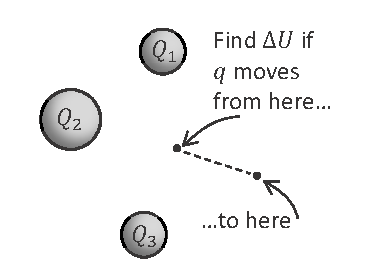
\includegraphics[scale=0.8]{potential_intro/activity_3_figs/charge_from_pocket_potential.eps}
\end{center}
\end{wrapfigure}
speed of the charge $q$ from your pocket?  You could calculate the electric potential energy at the initial and final positions, and find the change in kinetic energy using $\Delta K = -\Delta U$.

But again, the size of $\Delta U$ depends on what charge $q$ you pull from your pocket, and you might not want to recalculate it from scratch for every possible charge you could pull out.  Instead, you can calculate a new quantity called the ``electric potential'' $V$ at the initial and final positions.  Just as $E$ tells you the force per unit charge $q$, this new quantity $V$ tells you the ``potential energy per unit charge'' for whatever new charge $q$ you put down.  The electric potential is defined as:
$$V \equiv \frac{U}{q}$$
\vspace{-0.3 in}
\begin{enumerate}[labparts]

\item Go ahead and fill in the missing equation on the diagram below, analogous to the previous diagram with $\vv{F}$ and $\vv{E}$.  (It seems a little silly here, but play along anyway; the payoff is coming on the next page!)
\begin{center}
\includegraphics{potential_intro/concept_map_figs/concept_map_U_and_V_blank.eps}
\end{center}

\item Note that the name ``electric potential'' makes it sound like $V$ is an energy, but it's not.  (Even more confusing: the electric potential $V$ is sometimes called just ``the potential'' for short.)  What are the SI units for potential energy $U$?  
\answerspace{0.3in}

\item By contrast, what would be the units of electric potential $V$, in terms of SI units you already know?  (This unit is also defined as the Volt, and is abbreviated as ``V''.)
\answerspace{0.3in}

\end{enumerate}

\pagebreak[2]
\textbf{Activity 3: A Quick Example Problem}

Let's do a quick example problem to show how handy the electric potential $V$ can be.  
\begin{quote}
\textbf{Problem:} An ionized helium atom has mass $m=6.7\times 10^{-27}$~kg and charge $q_0=+1.6\times 10^{-19}$~C.  It is released from rest at a place where the electric potential is $V = 80$~Volts.  (1 Volt = 1 Joule/Coulomb.)  The ion accelerates to a final location where the electric potential is $V= 25$~Volts.  What is the final speed $v_F$ of the helium ion?  
\end{quote}
\begin{enumerate}[labparts]
\item Find the change in the electric potential $\Delta V$ for the helium ion.  (Be careful with your signs!)
\answerspace{0.3in}

\item Find the change in the helium ion's potential energy $\Delta U$.  
\answerspace{0.3in}

\item What is the change in the helium ion's kinetic energy, $\Delta K$? 
\answerspace{0.3in}

\item What is the final speed $v_F$ of the helium ion?
\answerspace{0.6in}

\end{enumerate}
\textit{Note that in this problem the electric potential at the two locations was given to you; you'll learn how to calculate $V$ on your own soon enough.}

\bigskip
\textbf{Activity 4: Relating Electric Field and Electric Potential}

The relationship between the electric field $\vv{E}$ and electric potential $V$ is exactly analogous to that between force $\vv{F}$ and potential energy $U$.  

\begin{enumerate}[labparts]

\item The diagram below shows the relationships between $\vv{F}$, $\vv{E}$, $U$, and $V$.\footnote{Technically, the exact notation $F=-\frac{dU}{ds}$ in the diagram is only applicable for the one-dimensional case.}
Fill in the equations between $\vv{F}$ and $\vv{E}$ and between $U$ and $V$ from memory if you can.  Then write the two relationships between $\vv{E}$ and $V$.  Hint: start with the analogous equations relating $\vv{F}$ and $U$, and divide both sides by $q$.  
\begin{center}
\includegraphics{potential_intro/concept_map_figs/concept_map_all_blanks.eps}
\vspace*{0.2in}
\end{center}

\item The graph below shows the electric potential $V$ along the $x$ axis.  Draw a qualitative graph showing the potential energy $U(x)$ for a \textit{positively} charged particle placed on the $x$ axis.  \label{part_potential_intro_given_V}

\begin{lab_axis}*[lab_noticks_2quads,
	width={2.7in}, height={1.6in},
	algebraic_labels,
	xlabel={$x$},
	ylabel={$V$},
	xmax={6},
	xtick={2,4},
	xticklabels = { , },
	]
\addplot coordinates {(0,0) (2,0.8) (4,0.8) (5,0) (5.5,0) };
\end{lab_axis}

\begin{lab_axis}*[lab_noticks_2quads,
	width={2.7in}, height={1.6in},
	algebraic_labels,
	xlabel={$x$},
	ylabel={$U$},
	xmax={6},
	xtick={2,4},
	xticklabels = { , },
	]
\end{lab_axis}

%\begin{center}
%%\vspace{-0.1 in}
%\includegraphics{potential_intro/activity_5_figs/given_V.eps}
%
%\vspace{-0.1 in}
%\includegraphics{potential_intro/activity_5_figs/U_axes.eps}
%%\vspace{-0.1 in}
%\end{center}

\item For the graph of $V(x)$ given in part \ref{part_potential_intro_given_V}, draw a qualitative graph showing the potential energy  $U(x)$ for an \textit{electron} placed on the $x$ axis.
%\begin{center}
%\vspace{-0.1 in}
%\includegraphics{potential_intro/activity_5_figs/U_axes.eps}
%%\vspace{-0.1 in}
%\end{center}
\begin{lab_axis}*[lab_noticks_2quads,
	width={2.7in}, height={1.6in},
	algebraic_labels,
	xlabel={$x$},
	ylabel={$U$},
	xmax={6},
	xtick={2,4},
	xticklabels = { , },
	]
\end{lab_axis}

%\newpage
\item  For the graph of $V(x)$ given in part \ref{part_potential_intro_given_V}, sketch a qualitative graph of $\vv{E}(x)$.
%\begin{center}
%%\vspace{-0.1 in}
%\includegraphics{potential_intro/activity_5_figs/E_axes.eps}
%%\vspace{-0.1 in}
%\end{center}

\begin{lab_axis}*[lab_noticks_2quads,
	width={2.7in}, height={1.6in},
	algebraic_labels,
	xlabel={$x$},
	ylabel={$E$},
	xmax={6},
	xtick={2,4},
	xticklabels = { , },
	]
\end{lab_axis}

\pagebreak[3]
\item The figure below shows electric field vectors in a region of space.  In traveling  along each of the dotted-line paths below, is the change in electric potential $\Delta V$ \textit{positive},  \textit{negative}, or  \textit{zero}?  (Think: if pushing a positive charge $+q$ along the path with your hand would require doing \textit{positive} work, then you would  be \textit{increasing} the potential energy of the system.)
\begin{center}
\vspace{-0.1 in}
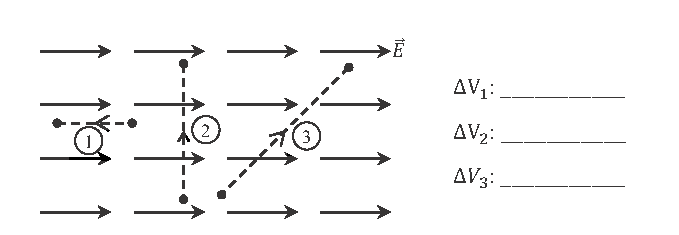
\includegraphics{potential_intro/activity_5_figs/uniform_E_field_1.eps}
\end{center}

%\item The figure below shows a region of space with a uniform electric field.  Draw two different dotted line paths, each of which has constant electric potential along the path.  Which of your two paths is at a higher electric potential?  (Each of these paths is called an ``equipotential''.)
\item  One of the three paths  above is an ``equipotential,'' meaning that every point along the path has the same electric potential $V$.  The figure below shows another region of space with a uniform electric field.  Draw two dotted line paths showing equipotentials on the figure below.  Which of your two paths is at a higher electric potential?

\begin{center}
\vspace{-0.25 in}
\includegraphics{potential_intro/activity_5_figs/uniform_E_field_2_squish.eps}
\end{center}

\item The figure below shows the electric field lines around a positively charged particle.  Draw two different dotted lines (actually curves) representing equipotentials.  Label which of your two equipotential lines has a higher electric potential and which one has a lower electric potential. 
\begin{center}
\vspace{-0.1 in}
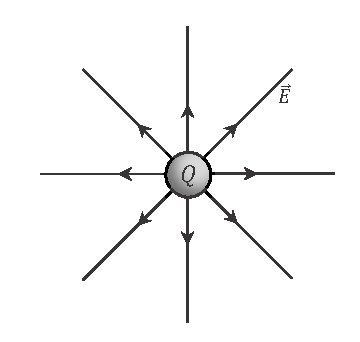
\includegraphics{potential_intro/activity_5_figs/point_charge_E_field.eps}
\end{center}

%\newpage
%\pagebreak[4]
\item The drawing below shows a region of uniform electric field.  Draw a qualitative graph of $V(x)$ along the dotted line shown, defining the potential at point B to be $V=0$.  To check your answer, compare your graph with those you drew in Activity 2.  \label{part_potential_intro_draw_V} 

\begin{center}
\includegraphics{potential_intro/activity_5_figs/uniform_E_field_3.eps}
\hspace{0.5in}
\begin{lab_axis}[lab_noticks_2quads,
	algebraic_labels,
	width={1.7in}, height={1.6in},
	xlabel={$x$},
	ylabel={$V$},
	xtick={0.2, 0.6, 0.8},
	xticklabels = {C, B, A},
	]
\end{lab_axis}
\end{center}


\end{enumerate}

\textbf{Activity 5: The Electric Potential of a Point Charge}

In part \ref{part_potential_intro_draw_V} of the previous activity, you essentially found $V$ by integrating the electric field, using
$$V=-\int{\vv{E} \cdot \vv{ds}}.$$
Now let's apply this same relationship to one of the most common situations you've seen so far: a single point charge.  We'll put a positive point charge $+Q$ at the origin, at $r=0$, and find the electric potential $V(r)$ due to that point charge.
\begin{center}
\vspace{-0.1 in}
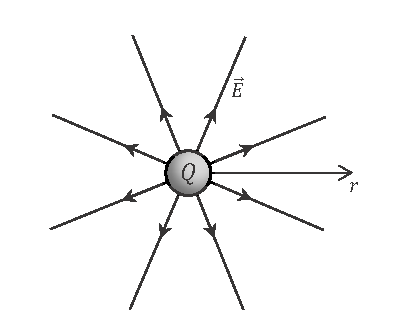
\includegraphics{potential_intro/activity_6_figs/point_charge_E_field_axis.eps}
\end{center}

\begin{enumerate}[labparts]

\item Before we do any calculations, we'll try to get a general feel for what $V(r)$ should look like.  Imagine taking a small charge $q$ out of your pocket, and pushing it in towards $r=0$ from $r=\infty$.  (We'll assume $q$ is positive, so that $U$ and $V$ have the same sign.)  As you push $q$ inward with your hand, does the electric potential due to $Q$ \textit{increase}, \textit{decrease}, or \textit{stay the same} as you get closer to $Q$?
\answerspace{0.4in}

\item The electric field from $Q$ gets stronger as you get closer.  Bearing in mind that $E = -dV/dr$, is the magnitude $\left | {dV}/{dr}\right |$ getting bigger or smaller as you get closer to $Q$?
\answerspace{0.4in}

\item Based on your last two answers, sketch a qualitative graph of $V(r)$ on the axes below.  For convenience, let $V=0$ at $r \rightarrow \infty$. \label{part_potential_intro_sketch_of_Vr}
%\begin{center}
%\includegraphics{potential_intro/activity_6_figs/V_axes.eps}
%\end{center}
\begin{lab_axis}*[lab_noticks_2quads,
	width={2.2in}, height={1.9in},
	algebraic_labels,
	xlabel={$r$},
	ylabel={$V$},
	]
\end{lab_axis}

\pagebreak[2]
\item Now that we have some intuition about what $V(r)$ should look like, let's actually do the calculation.  First, write the electric field $E(r)$ at a distance $r$ from the charge in terms of $Q$, $r$, and the Coulomb constant $k_e$.
\answerspace{0.5in}

\item Since the $\vv{E}$ points radially outward, the equation $V=-\int{\vv{E} \cdot \vv{ds}}$ can be reduced to 
the one-dimensional form $V=-\int{E \, dr}$.  Perform that integration to find $V(r)$, using the $E(r)$ you just wrote. Be sure to include an integration constant $+C$.
\answerspace{1.2in}

\item As with the potential energy $U$, you're free to set $C$ to whatever value you want, since the only \textit{physical} meaning of $V$ comes when we take the difference $\Delta V$ between two points.  It's often convenient to set our ``reference value'' of $V$ so that $V=0$ at $r \rightarrow \infty$.  What value of $C$ makes that true?
\answerspace{0.5in}

\item Does your answer for $V(r)$ match with your graph from part \ref{part_potential_intro_sketch_of_Vr}?
\answerspace{0.5in}

%\item draw E(x) along x-axis.  (signs)  Note: save this for the second electric potential lab.

%\item draw V(x) along x-axis.  Check that E = -dV/ds.

\end{enumerate}

You should have found that the electric potential $V$ for a point charge $Q$ is given by
$$V=\frac{k_eQ}{r},$$
where $k_e$ is the Coulomb constant.  The form looks very similar to that of the electric field for a point charge, $E={k_eQ}/{r^2}$, and quick pencil sketches of the two functions tend to look identical.  But of course the two don't have the same units, and the \textit{meaning} of $\vv{E}$ and $V$ are very different---just as distinct as their analogs, $\vv{F}$ and $U$.  
  




\section{The Electric Potential for Multiple Charges: Superposition}
\label{potential_superposition}

\instructornote{%
By Matt, Spring 2017.  Time: Long, $\sim$80 minutes(?)

Students find this lab very difficult!
}

\makelabheader %(Space for student name, etc., defined in master.tex)

\bigskip

\textbf{Introduction} 

In this lab, you will practice visualizing $\vv{E}$ and $V$ for several point charges, using the idea of superposition.

\textbf{Apparatus}

\begin{itemize}[nosep]
\item An internet browser with access to Paul Falstad's 2-D Electrostatic Fields Applet
\end{itemize}

\bigskip

\textbf{Activity 1: \textit{E} and \textit{V} For a Single Point Charge}

Open an internet browser and go to \verb!http://www.falstad.com/vector2de/fullscreen.html!.  It may take a few moments to load, but eventually you'll see a graphic of a bunch of dots falling into a funnel.  There's a lot going on here, so follow these steps to simplify the display:
\begin{itemize}[nosep]
\item On the first menu (``Setup'') select the fifth item down, \verb!Setup: point charge!
\item On the third menu (``Floor'') select \verb!Floor: grid!
\item For ``Display'' select \verb!Display: None!
\item Check the box next to \verb!Reverse!
\item For the ``Mouse'' menu, you may want to select \verb!Mouse = Adjust Zoom!, then hold the left button down and move the mouse left and right to adjust the size of the display.  When it seems reasonably sized, return the menu to \verb!Mouse = Adjust Angle!
\end{itemize}

The surface you see represents the electric potential $V$ for a positive point charge located at the origin, as you studied in the final activity of Lab~\ref{potential_intro}.  The height of the surface on the $z$-axis represents the value of $V(x,y)$.  Use the mouse to adjust the viewing angle to get a sense of the shape of the surface.  Cool, eh?  :-)

\begin{enumerate}[labparts]

\item Imagine walking in a straight line path along the $x$ axis ($y=0$), directly past the positive charge at the origin.  On the axes below, sketch a graph of the electric potential $V(x)$ along your path.  
%\begin{center}
%\vspace{-0.1in}
%\includegraphics{potential_superposition/activity_1_figs/V_axes.eps}
%\vspace{-0.1in}
%\end{center}

%\vspace{-0.1in}
\begin{lab_axis}*[lab_noticks_4quads,
	width={3.0in}, height={1.7in},
	xlabel=$x$,
	ylabel=$V$,
	]
\end{lab_axis}

\item On the axes below, sketch a graph of the electric field $E_x(x)$ for along the $x$ axis.  Remember, the \textit{sign} of $E_x$ represents the direction of the field.  (Think: which direction does $\vv{E}$ point on the left side and right side of the charge?
%\begin{center}
%\vspace{-0.1in}
%\includegraphics{potential_superposition/activity_1_figs/E_axes.eps}
%\vspace{-0.1in}
%\end{center}

\begin{lab_axis}*[lab_noticks_4quads,
	width={3.0in}, height={1.7in},
	xlabel=$x$,
	ylabel=$E_x$,
	]
\end{lab_axis}


\item The signs of your graph should be consistent with 
%the relationship
$\displaystyle E_x=-\frac{dV}{dx}$. Are they?\footnote{Actually, for more than one dimension, a better notation is to use partial derivatives: 
$\displaystyle E_x=-\frac{\partial V}{\partial x}$,  
$\displaystyle E_y=-\frac{\partial V}{\partial y}$, and 
$\displaystyle E_x=-\frac{\partial V}{\partial z}$.
In fact, $\vv{E}=-\nabla V$.  (If you haven't had multivariate calculus yet, you can ignore this.)}
\answerspace{0.3in}

\item Looking at the 3D surface, does the electric field point \textit{uphill} or \textit{downhill?}
\answerspace{0.3in}

\item Write the mathematical functions for $V(x)$ and $E(x)$ along the positive $x$ axis ($x > 0$).  Are they the same?
\answerspace{0.3in}

%View equipotentials?
\end{enumerate}

\textbf{Activity 2: \textit{E} and \textit{V} For Two Positive Point Charges: Superposition}

Now suppose we have two identical positively charge particles, $Q_1$ and $Q_2$, located on the $x$ axis at $x= \pm a$ as shown below.
%\begin{center}
%\vspace{-0.1in}
%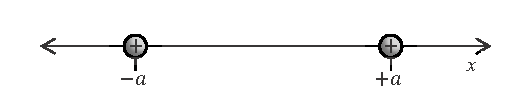
\includegraphics{potential_superposition/activity_2_3_figs/charges_on_x_axis.eps}
%\vspace{-0.1in}
%\end{center}

\begin{lab_axis}*[lab_noticks_1axis,
	xtick={-0.4,+0.4},
	xticklabels={$-a$,$+a$},
	xtick pos=left,
	tick style={major tick length=15pt},
	tick label style = {font=\itshape},
	]
\addplot [only marks, line width=0.5pt, mark = ball, mark size=6pt, ball color=white] coordinates {(-0.4, 0) (0.4, 0)};
% The preceding line generates a warning:
%	"Package pgf Warning: No path specified that can be filled on input line [....]"
% It seems to be the "ball color=white" part that it doesn't like.  I have no idea why.
\addplot [only marks, mark = +, mark size=4pt, line width=2pt] coordinates {(-0.4, 0) (0.4, 0)};
\end{lab_axis}

%Below, I decided not to use \vv{F}\!_{NET}
Any additional charge $q$ you take out of your pocket will feel the net force $\vv{F}$ due to both $Q_1$ and $Q_2$:
$$\vv{F} = \vv{F_1} + \vv{F_2}.$$
You can divide both sides of the equation above by $q$ to show that the electric fields due to $Q_1$ and $Q_2$ add the same way.  We call this idea \textit{superposition}:
$$\vv{E} = \vv{E_1} + \vv{E_2}.$$
You can take $-\int \vv{ds}$ of both sides to show that you can also use superposition to combine electric potentials:
\begin{align*}
-\int{\vv{E} \cdot \vv{ds}} %&= -\int{\left (\vv{E_1} + \vv{E_2} \right) \cdot \vv{ds}} \\
&= -\int{\vv{E_1} \cdot \vv{ds}} + -\int{\vv{E_2} \cdot \vv{ds}} \\
V &= V_1 + V_2
\end{align*}

\begin{enumerate}[labparts]

\item On the axes below, make a prediction for the electric potential $V(x)$ along the $x$ axis due to the two point charges pictured above.  Use dotted lines to show the electric potentials $V_1$ and $V_2$ due to the two individual charges, and use a solid line to show the resulting net electric potential $V$.  
%\begin{center}
%\vspace{-0.1in}
%\includegraphics{potential_superposition/activity_2_3_figs/V_axes.eps}
%\vspace{-0.1in}
%\end{center}

\begin{lab_axis}*[lab_noticks_4quads,
	width={3.0in}, height={1.7in},
	xlabel=$x$,
	ylabel=$V$,
	xtick={-0.4,+0.4},
	xticklabels={$-a$,$+a$},
	tick label style = {font=\itshape},
	]
\end{lab_axis}

\item Use the computer program to see how you did.  On the first menu, choose \verb!setup: point charge double!.  You'll also have to re-click the box marked \verb!Reverse! to show \textit{positive} charges.  Use the mouse to adjust the scale and the angle as before.  Does what you see match your prediction?
\answerspace{0.3in}

\textit{Make any changes you need to make on your graphs on the previous page.}

\item On the axes below, draw a sketch of the electric field $E(x)$ along the $x$ axis.  Again, use dotted lines to show $E_1$ and $E_2$ due to the two individual charges, and a solid line to show the net electric field $E$.
%\begin{center}
%\vspace{-0.1in}
%\includegraphics{potential_superposition/activity_2_3_figs/E_axes.eps}
%\vspace{-0.1in}
%\end{center}

\begin{lab_axis}*[lab_noticks_4quads,
	width={3.0in}, height={1.8in},
	xlabel=$x$,
	ylabel=$E_x$,
	xtick={-0.4,+0.4},
	xticklabels={$-a$,$+a$},
	tick label style = {font=\itshape},
	]
\end{lab_axis}


\item Is $V=0$ at $x=0$?
\answerspace{0.3in}

\item Is $E=0$ at $x=0$?
\answerspace{0.3in}

\textit{Rotate the graph on the screen to view a profile of $V(x)$ from the side.  (You'll be looking directly along the $y$ axis.)  Check to be sure your two answers above are consistent with the surface you see at $x=0$.}

\item  Change the third menu item to select \verb!Floor: equipotentials!.  On the $x$ and $y$ axes below, use dotted lines to sketch the equipotentials you see.  Then, using solid lines, draw in electric field lines for the two charges.  (One-word hint: \textit{perpendicular}.)
%\begin{center}
%\vspace{-0.1in}
%\includegraphics{potential_superposition/activity_2_3_figs/x_y_axes.eps}
%\vspace{-0.1in}
%\end{center}

\begin{lab_axis}*[lab_noticks_4quads,
	width={3.0in}, height={1.8in},
	xlabel=$x$,
	ylabel=$y$,
	xtick={-0.4,+0.4},
	xticklabels={$-a$,$+a$},
	tick label style = {font=\itshape},
	]
\end{lab_axis}


\end{enumerate}

\pagebreak[3]
\textbf{Activity 3: \textit{E} and \textit{V} For a Dipole}

Hmmm.... What would our graphs look like if one of the charges were negative, as shown below?  (This configuration of equal and opposite charges is called a dipole.)
%\begin{center}
%\vspace{-0.1in}
%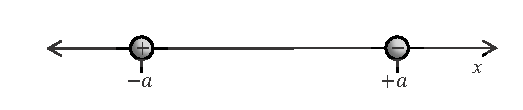
\includegraphics{potential_superposition/activity_2_3_figs/charges_on_x_axis_dipole.eps}
%\vspace{-0.1in}
%\end{center}

\begin{lab_axis}*[lab_noticks_1axis,
	xtick={-0.4,+0.4},
	xticklabels={$-a$,$+a$},
	xtick pos=left,
	tick style={major tick length=15pt},
	tick label style = {font=\itshape},
	]
\addplot [only marks, line width=0.5pt, mark = ball, mark size=6pt, ball color=white] coordinates {(-0.4, 0) (0.4, 0)};
\addplot [only marks, mark = +, mark size=4pt, line width=2pt] coordinates {(-0.4, 0)};
\addplot [only marks, mark = -, mark size=4pt, line width=2pt] coordinates {(+0.4, 0)};
\end{lab_axis}



\begin{enumerate}[labparts]

\item As before, make a prediction below for the electric potential $V(x)$ along the $x$ axis due to the two point charges pictured above.  Use dotted lines to show the electric potentials $V_1$ and $V_2$ due to the two individual charges, and use a solid line to show the resulting net electric potential $V$.  
%\begin{center}
%\vspace{-0.1in}
%\includegraphics{potential_superposition/activity_2_3_figs/V_axes.eps}
%\vspace{-0.1in}
%\end{center}

\begin{lab_axis}*[lab_noticks_4quads,
	width={3.0in}, height={1.8in},
	xlabel=$x$,
	ylabel=$V$,
	xtick={-0.4,+0.4},
	xticklabels={$-a$,$+a$},
	tick label style = {font=\itshape},
	]
\end{lab_axis}

\item On the axes below, draw a sketch of the electric field $E(x)$ along the $x$ axis.  Again, use dotted lines to show $E_1$ and $E_2$ due to the two individual charges, and a solid line to show the net electric field $E$.
%\begin{center}
%\vspace{-0.1in}
%\includegraphics{potential_superposition/activity_2_3_figs/E_axes.eps}
%\vspace{-0.1in}
%\end{center}

\begin{lab_axis}*[lab_noticks_4quads,
	width={3.0in}, height={1.8in},
	xlabel=$x$,
	ylabel=$E_x$,
	xtick={-0.4,+0.4},
	xticklabels={$-a$,$+a$},
	tick label style = {font=\itshape},
	]
\end{lab_axis}

\item Use the visualization application to see how you did.  On the first menu, choose \verb!setup: dipole!.  This time you don't have to click the \verb!Reverse! box.  Does the surface you see match your predictions?
\answerspace{0.3in}

\item Is $V=0$ at $x=0$?
\answerspace{0.3in}

\item Is $E=0$ at $x=0$?
\answerspace{0.3in}

\textit{Again, rotate the graph on the screen to view a profile of $V(x)$ from the side.  Check to be sure your two answers above are consistent with the surface you see at $x=0$.}

\item On the axes below, sketch the equipotential curves for the dipole using dotted lines, and sketch the electric field lines using solid lines.
%\begin{center}
%\vspace{-0.1in}
%\includegraphics{potential_superposition/activity_2_3_figs/x_y_axes.eps}
%\vspace{-0.1in}
%\end{center}

\begin{lab_axis}*[lab_noticks_4quads,
	width={3.0in}, height={1.8in},
	xlabel=$x$,
	ylabel=$y$,
	xtick={-0.4,+0.4},
	xticklabels={$-a$,$+a$},
	tick label style = {font=\itshape},
	]
\end{lab_axis}

\item Suppose you took a positive charge $+q$ from your pocket, and moved it with your hand from $r=\infty$ to the origin, along the $y$ axis.  What is the direction of the electric force acting on the charge?
\answerspace{0.5in}

\item Would your hand do \textit{positive work}, \textit{negative work}, or \textit{zero work} in moving the charge in along the $y$ axis?
\answerspace{0.3in}
\end{enumerate}

\section{The Electric Potential for Continuous Charge Distributions}
\label{potential_charge_distributions}
\begin{comment}
This lab was written by Matt Trawick in January, 2017.  It incorporates some of the pieces from the original Workshop Physics lab from Dickinson College, but adds some material (potential for a finite rod), and removes some of the introductory stuff, which is now done elsewhere.
\end{comment}

\makelabheader %(Space for student name, etc., defined in master.tex)

\bigskip

\textbf{Introduction} 

You already know how to use the idea of superposition to find the potential due to a handful of point charges.  In this lab, you'll use the same basic idea to find the potential due to a \textit{continuous} distribution of charge, such as a long, uniformly charged rod or a uniformly charged ring.

\bigskip

\textbf{Activity 1: Numerical Approximation of \textit{V} Due to a Charged Rod}

\begin{minipage}{0.64\textwidth}
\begin{quote}
\textbf{Problem:} A thin rod of length $L=20$~cm, with a total positive charge $Q=10$~nC, lies on the $y$ axis between $y=0$ and $y=20$~cm.  Calculate the electric potential $V$ due to the rod at a point $P$ along the $x$ axis a distance x=15 cm from the origin. 
\end{quote}

\textbf{Solution:} In this activity, you will estimate $V$ numerically, using Excel.  Divide the rod into ten individual 1~nC pieces, which you can approximate as point charges located at $y=1$~cm, $y=3$~cm, etc., up to $y=19$~cm.  
\end{minipage}
\begin{minipage}{0.35\textwidth}
\vspace{-0.3in}
\raggedleft \includegraphics[scale=0.9]{potential_charge_distributions/rod_axes.eps}
\end{minipage}

\begin{enumerate}[wide, label=(\emph{\alph*})]

\item Use Excel to find the electric potential at point $P$ due to \textit{only} the furthest 1~nC point charge, located at $y=19$~cm.  Use $k_e=8.99 \times 10^9$~N$\cdot$m$^2/$C$^2$.  (\textit{Answer:} $\sim 37$ Volts.)
\answerspace{0.5in}

\item Create nine more rows in your Excel table for the other 1~nC charges.  What is the electric potential at point $P$ due to all of them?  (\textit{Answer:} $\sim 494$ Volts, but go ahead and write it to six significant figures.) 
\answerspace{0.5in}

\end{enumerate}

\begin{wrapfigure}[10]{r}{0.30\textwidth}
\includegraphics[scale=0.9]{potential_charge_distributions/rod_integral.eps}
\end{wrapfigure}
\textbf{Activity 2: Exact Calculation of \textit{V} Due to a Charged Rod}

Of course, you can imagine making your solution progressively more and more accurate by dividing the rod into smaller and smaller pieces.  And for some very difficult problems, this technique (called ``finite element'' analysis) is the only way to get an answer at all!  But for the thin rod, you can actually calculate an exact solution, by allowing the elements to become infinitely small and performing an integration.

Start by picking a small bit of charge dQ from an arbitrary place in the middle of the rod.  Instead of a discrete sum, you'll integrate
$$V=\int{\frac{k_e\,dQ}{r}}$$
adding up the contributions of each $dQ$ over the whole length of the rod.
\begin{enumerate}[wide, label=(\emph{\alph*})]

\pagebreak[2]
\item Write $dQ$ in terms of $L$, $Q$, and $dy$.
\answerspace{0.3in}

\item Write the distance $r$ from the $dQ$ to the point $P$ in terms the quantities given.  ($y$, $x$, or $L$...) 
\answerspace{0.4in}

\item Now write out the whole integral and solve it.  What are the limits of integration?  One of the integrals given on the right may be useful. \label{part_potential_charge_distributions_exact_rod}
%\answerspace{1.3in}

\begin{minipage}{0.65\textwidth}
\
\end{minipage}
\begin{minipage}{0.34\textwidth}

%\begin{raggedleft}
\textit{World's fourth smallest integral table:}
\begin{align*}
&\int \! \frac{1}{\left (u^2 + a^2 \right )^\frac{3}{2}} \, du=\frac{u}{a^2 \sqrt{u^2 + a^2}} \\
&\int \! \frac{u}{\left (u^2 + a^2 \right )^\frac{3}{2}} \, du=\frac{-1}{\sqrt{u^2 + a^2}} \\
&\int \! \frac{1}{u^2 + a^2} \, du=\frac{1}{a} \tan^{-1} \frac{u}{a} \\
&\int \! \frac{1}{\left (u^2 + a^2 \right )^\frac{1}{2}} \, du=\ln \left | u + \sqrt{u^2 + a^2} \right| \\
\end{align*}
%\end{raggedleft}
\end{minipage}
\item Compare your numerical answer in part \ref{part_potential_charge_distributions_exact_rod} to the answer you calculated in Activity 1.  How close are they, and which one is more precise?
\answerspace{0.4in}

\end{enumerate}

\textbf{Activity 3: Numerical Approximation of \textit{V} Due to a Charged Ring}
\footnote{Activities 3, 4, and 5 are based on previous work (1990-93) by the Department of Physics and Astronomy, Dickinson College. Supported by FIPSE (U.S. Dept. of Ed.) and NSF. Portions of this material were modified locally and have not been classroom tested at Dickinson College.}

\begin{minipage}{0.65\textwidth}
Let's take a look at another example problem, which we'll actually solve three different ways over the next three activities.  

\begin{quote}
\textbf{Problem:} A thin, uniformly charged ring of radius $a=30$~cm has a total charge of $Q = 20\ \mu$C ($20
\times 10^{-6}$~C). Find the electric potential $V$ at a point $P$ a distance $x = 20$~cm from the ring along an axis perpendicular to the ring, passing through its center.
\end{quote}

\textbf{Solution:} As in Activity 1, we will first estimate $V$ numerically, dividing the ring into 20 elements, each of charge $\Delta q = 1\ \mu$C.

\end{minipage}
\begin{minipage}{0.34\textwidth}
\vspace{-0.3in}
\raggedleft \includegraphics[scale=0.9]{potential_charge_distributions/ring_integral.eps}
\end{minipage}

\begin{enumerate}[wide, label=(\emph{\alph*})]

\item Find $V$ at the point $P$ due to \textit{just one} of the 20 elements.
\answerspace{0.4in}

\item Find $V$ at  point $P$ due to \textit{all} of the 20 elements combined.  You can either use Excel or calculate it by hand; in either case, summarize your procedure below.
\answerspace{0.7in}

\end{enumerate}

\pagebreak[2]
\textbf{Activity 4: Calculating \textit{V} Due to a Charged Ring Using an Integral}

Perhaps you found that your numerical calculation in the last part was fairly trivial---great!  Just for fun, let's see how the integral method for finding $V$ works in this case, and whether we get a more exact answer.

\begin{enumerate}[wide, label=(\emph{\alph*})]

\item Consider a small charge $dQ$ somewhere on the ring, referring back to the figure on the previous page.  Write the integral  
%$V=\int{({k_e/r})\,dQ}$
$\displaystyle V=\int{\frac{k_e\,dQ}{r}}$
with $r$ expressed in terms of quantities given in the figure.
\answerspace{0.6in}

\item The integral you've just written looks hard at first.  But think carefully about what's \textit{constant} in the integral you just wrote.  (What values would be unchanged for the next $dQ$ you choose?)  Rewrite your expression above, pulling any constants outside of the integral sign.
\answerspace{0.5in}

\item What you're left with should be a trivial integral.  Go ahead and solve it, computing a numerical answer for $V$ at $x = 20$~cm.
\answerspace{0.7in}


\item How does your answer above compare to your result in Activity 3?
\answerspace{0.3in}
\end{enumerate}

\textbf{Activity 5: Calculating \textit{V} for the Ring From the Electric Field}

\bigskip

\begin{minipage}{0.60\textwidth}
So far you've found the electric potential for charge distributions using 
%$V=\int{({k_e/r})\,dQ}$
$\displaystyle V=\int{\frac{k_e\,dQ}{r}}$.  
But you also know that 
%$V$ is related to the electric field by 
%$V=-\int{\vv{E} \cdot \vv{ds}}$.  
$\displaystyle V=-\int{\vv{E} \cdot \vv{ds}}$.  
In this activity, we'll find $V$ for the ring a new way: by calculating $\vv{E}$ first, and then getting $V$ from there.

\begin{enumerate}[wide, label=(\emph{\alph*})]

\item What is the direction of $\vv{E}$ at point $P$ due to the \textit{whole} ring?
\answerspace{0.3in}

\item Referring to the figure to the right, write an expression for the magnitude $| \vv{dE} |$ of the electric field due to just a single bit of charge $dQ$.

\end{enumerate}
\end{minipage}
\begin{minipage}{0.39\textwidth}
\vspace{-0.3in}
\raggedleft 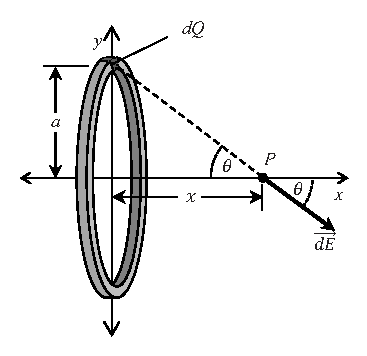
\includegraphics[scale=1.0]{potential_charge_distributions/ring_E_field.eps}
\end{minipage}
$$| \vv{dE}|=\hspace{0.7in}$$
\answerspace{0.1in}

\begin{enumerate}[wide, label=(\emph{\alph*}), start=3]

\item When you add up all of the $\vv{dE}$ from each $dQ$, the $y$ and $z$ components all cancel, leaving only $dE_x$.   What is the magnitude of $dE_x$?  (It should be similar to your answer above, but multiplied by either $\sin \theta$ or $\cos \theta$.)

$$dE_x=\hspace{0.7in}$$
\answerspace{0.1in}

\pagebreak[2]
\item Rewrite the last step, giving  $\sin \theta$ or $\cos \theta$ in terms of a ratio involving $x$, $a$, and/or $\sqrt{x^2 + a^2}$.

$$dE_x=\hspace{0.7in}$$

\medskip

\item Write the complete integral expression for $\vv{E}$.  As in the previous activity, many things inside the integral are actually constant, leaving you with yet another trivial integral to solve.  Solve the integral, and write below a final expression for $\vv{E}$ at an arbitrary point $x$ along the axis.  
\answerspace{0.8in}

\item Now that you have $E$ for every point along the axis, you can integrate it to find $V = - \int{E \, dx}$.  This integral is definitely \textit{not} trivial, but you may find one of the integrals in the table on \pageref{part_potential_charge_distributions_exact_rod} to be helpful.  (Don't forget the integration constant, $+C$.  What will you use for $C$, and why?)
%\answerspace{1.0in}
\vfill

\item Does your answer match with what you found in activities 3 and 4?
\answerspace{0.3in}

\end{enumerate}

\textbf{A General Note About Different Methods For Finding \textit{V}}

In this lab, we used two general methods for finding $V$ from a charge distribution:

\begin{quote}
\textbf{Method 1:} (Activities 1 -- 4) Calculate $V$ directly, using either
$$V = \sum_i{\frac{k_e Q_i}{r_i}}
\qquad  \mathrm{or} \qquad  
V = \int{\frac{k_e \, dQ}{r}}$$
\end{quote}

\begin{quote}
\textbf{Method 2:} (Activity 5) First calculate $\vv{E}$, perhaps using either
$$E = \sum_i{\frac{k_e Q_i}{r^2}}
\qquad  \mathrm{or} \qquad 
\vv{E} = \int{\frac{k_e \, dQ}{r^2}\hat{r}}$$
\phantom{\textbf{Method 2:} }Then find $V$ from $\vv{E}$ using
$$V = - \int{\vv{E} \cdot \vv{ds}}$$
\end{quote}

Both work!  But it should be clear just from the descriptions above that method 2 is going to be a much bigger pain in the badonkadonk most of the time.  (For one thing, method 2 requires two integrals instead of one, and it also requires finding the \textit{vector} $\vv{E}$, which means you have to deal with multiple components.)  Method 1 is almost always your best choice.  The only exception when you might choose method 2 is if you already know $\vv{E}$ or can calculate it relatively easily, for instance by using Amp\`ere's law.




\section{Magnetism: Measuring Field from Current in a Straight Wire}

\makelabheader %(Space for student name, etc., defined in master.tex)


\bigskip
\textbf{Apparatus} 

\begin{itemize} [nosep]
\item Power supply
\item Long banana wire 
\item Stand and clamps for holding wire vertically
\item Teeny-weeny compass
\end{itemize}

\bigskip
\textbf{Activity}

Before you do anything else, verify that your teeny-weeny compass actually works.  It should point north when it's far away from any magnets or steel.  

\begin{enumerate}[labparts]

\item Make a prediction: will electric current in a wire produce a magnetic field that will deflect your compass?  If so, what direction will the magnetic field point?  (Radially inwards, towards the wire?  Away from the wire?  Circumferentially around the wire?)
\answerspace{0.5 in}

Set up your equipment to do the experiment, connecting the power supply so that positive current travels \textit{up} the vertical wire.  Crank the current up all the way so that the display reads just over 3 Amps.  

\item Hold the teeny-weeny compass very close to the vertical section of the wire, so that the outside of the compass  actually \textit{touches} the wire's rubber insulation.  Move the compass on all sides of the wire (in front, behind, etc.).  Based on your observations, describe the apparent direction of the magnetic field near the wire. \label{part_straight_wire_regular}
\answerspace{0.5 in}

\item By pointing north, your compass is pointing \textit{in the direction} of the local magnetic field.  As you look down on the vertical wire from above, does the magnetic field seem to point \textit{clockwise} or \textit{counterclockwise} around the wire? 
\answerspace{0.3 in}

\item Make a prediction: what do you think will happen to the magnetic field when you reverse the direction of the current in the vertical wire, so that current travels \textit{down} instead of \textit{up}? \label{part_straight_wire_reversed}

\bigskip
\hspace{0.5in} Prediction:

\bigskip
\hspace{0.5in} Experiment:
\bigskip

\item The direction of the magnetic field is supposed to obey the following ``right-hand rule:''
\begin{quote}\textit{If you grab a wire with your right hand, with your thumb pointing in the direction of the current, your fingers should wrap around the wire in the direction of the magnetic field.}
\end{quote}
Are the results of your experiments in parts \ref{part_straight_wire_regular} and \ref{part_straight_wire_reversed} both consistent with this right-hand rule?
\answerspace{0.3 in}

\end{enumerate}


 

%--------------------------------------------
\appendix
\setcounter{section}{4} %set this counter to number MINUS ONE corresponding to desired appendix letter. (4 for `E', etc.)
%Put include statements for supplementary appendices below here.
\end{document}
